\section{同调正合列}
\sourcepage{151--152}
绝对同调与相对同调之间的关系由所谓“偶的同调正合列”表述。本节研究群的正合列，通常是阿贝尔群，并定义偶的同调正合列。

\entry{定义}{3.2.1}考虑有限或无限的群与同态序列 $\cdots\to A_1\xrightarrow{\varphi_1}A_2\xrightarrow{\varphi_2}A_3\to\cdots$。若 $\operatorname{im}\varphi_1=\ker\varphi_2$，则称在 $A_2$ 处\textbf{正合}（exact）。若在每个群处都正合，则称为\textbf{正合列}（exact sequence）。若序列有首项或末项，则不在这些端点定义正合性。

下个引理的各项应当已很熟悉，证明留作习题。因为只考虑阿贝尔群，以 $0$ 表示单元素平凡群。

\entry{引理}{3.2.2}有下列事实：
\begin{enumerate}[label=(\arabic*)]
\item $A_1\xrightarrow{\varphi}A_2\to0$ 正合，当且仅当 $\varphi$ 满射。
\item $0\to A_1\xrightarrow{\varphi}A_2$ 正合，当且仅当 $\varphi$ 单射。
\item 若 $0\to A_1\xrightarrow{\varphi}A_2\xrightarrow{\psi}A_3\to0$ 正合，称为\textbf{短正合列}（short exact sequence）。$\psi$ 诱导 $A_2/\varphi(A_1)\cong A_3$。反过来，若 $\psi:A\to B$ 满射，核为 $K$，则 $0\to K\xrightarrow{i}A\xrightarrow{\psi}B\to0$ 正合，$i$ 为包含。
\item 若 $A_1\xrightarrow{\alpha}A_2\xrightarrow{\varphi}A_3\xrightarrow{\beta}A_4$ 正合，则以下等价：(i) $\alpha$ 满射；(ii) $\beta$ 单射；(iii) $\varphi$ 为零同态。
\item 若 $A_1\xrightarrow{\alpha}A_2\to A_3\to A_4\xrightarrow{\beta}A_5$ 正合，则诱导序列 $0\to\operatorname{cok}\alpha\to A_3\to\ker\beta\to0$ 也正合。
\end{enumerate}

\entry{定义}{3.2.3}设两列群和同态 $\cdots\to A_i\to A_{i+1}\to\cdots$、$\cdots\to B_i\to B_{i+1}\to\cdots$ 的指标集相同。从前者到后者的\textbf{序列同态}是一族同态 $\alpha_i:A_i\to B_i$，使每个相应方块可交换，即沿横向同态再作用 $\alpha_{i+1}$，等于先作用 $\alpha_i$ 再沿下列横向同态。若每个 $\alpha_i$ 都是同构，称为\textbf{序列同构}。

例如，将链复形看作群与同态的序列，则序列同态恰好是链映射。

\entry{定义}{3.2.4}若短正合列 $0\to A_1\xrightarrow{\varphi}A_2\xrightarrow{\psi}A_3\to0$ 满足 $\varphi(A_1)$ 是 $A_2$ 的直和项，则称此列\textbf{分裂}（split）。

也就是说，$A_2=\varphi(A_1)\oplus B$，其中 $B$ 一般不唯一。$\varphi$ 给出 $A_1\cong\varphi(A_1)$，$\psi$ 给出 $B\cong A_3$。等价地，存在同构 $\theta:A_2\to A_1\oplus A_3$，使
\[
\begin{array}{ccccccccc}
0&\to&A_1&\xrightarrow{\varphi}&A_2&\xrightarrow{\psi}&A_3&\to&0\\
&&\Vert&&\downarrow\scriptstyle\theta&&\Vert\\
0&\to&A_1&\xrightarrow{i}&A_1\oplus A_3&\xrightarrow{\pi}&A_3&\to&0
\end{array}
\]
可交换，其中为外直和，$i$ 是包含，$\pi$ 是投影。$\theta$ 在第一直和项上取 $\varphi^{-1}$，在第二项上取 $\psi$。

\sourcepage{153--154}
\entry{定理}{3.2.5}对上述短正合列，下列条件等价：
\begin{enumerate}[label=(\arabic*)]
\item 此列分裂。
\item 存在同态 $p:A_2\to A_1$，使 $p\varphi=i_{A_1}$。
\item 存在同态 $j:A_3\to A_2$，使 $\psi j=i_{A_3}$。
\end{enumerate}
\noindent\textbf{证明：}(1) 蕴含 (2)、(3)：只需对标准列 $0\to A_1\to A_1\oplus A_3\to A_3\to0$ 验证。取 $p$ 为投影，$j$ 为包含即可。

(2) 蕴含 (1)：证明 $A_2=\varphi(A_1)\oplus\ker p$。每个 $x\in A_2$ 可写成 $x=\varphi p(x)+(x-\varphi p(x))$，前项在 $\varphi(A_1)$，后项在 $\ker p$，因为 $p(x-\varphi p(x))=p(x)-(p\varphi)p(x)=0$。若 $x\in\varphi(A_1)\cap\ker p$，写作 $x=\varphi(y)$，则 $0=p(x)=p\varphi(y)=y$，故 $x=0$。

(3) 蕴含 (1)：证明 $A_2=\ker\psi\oplus j(A_3)$，因为 $\ker\psi=\operatorname{im}\varphi$。写作 $x=(x-j\psi(x))+j\psi(x)$。前项在核中，因为 $\psi(x)-(\psi j)\psi(x)=0$；后项显然在像中。若 $x=j(z)$ 也在核中，则 $0=\psi(x)=\psi j(z)=z$，所以 $x=0$。\hfill$\square$

\entry{推论}{3.2.6}若短正合列的末端群 $A_3$ 自由阿贝尔，则此列分裂。

\noindent\textbf{证明：}选择 $A_3$ 的一组基。对每个基元素 $e$，从非空集合 $\psi^{-1}(e)$ 中选取一个元素作为 $j(e)$，再唯一扩张为同态 $j$，满足 $\psi j=i$。\hfill$\square$

现在可描述偶的同调正合列。先定义由边界算子诱导的\textbf{同调边界同态}
\[
\partial_*:H_p(K,K_0)\to H_{p-1}(K_0).
\]
给定相对闭链 $z\in C_p(K,K_0)$，它是某条 $K$ 的链 $d$ 模 $C_p(K_0)$ 的陪集，且 $\partial d$ 由 $K_0$ 承载。$\partial d$ 自动为 $K_0$ 的闭链，定义 $\partial_*\{z\}=\{\partial d\}$，花括号表示同调类。将在引理 3.3.2 证明中说明良定义性。

代数上，令 $i:K_0\to K$、$\pi:(K,\varnothing)\to(K,K_0)$ 为包含。$i_\#$ 是链群的包含，$\pi_\#$ 是商投影。给定相对闭链 $z$，先选择 $d$ 使 $\pi_\#d=z$，取边界 $\partial d$，它等于 $i_\#c$，其中 $c\in C_{p-1}(K_0)$ 为闭链。定义 $\partial_*\{z\}=\{c\}$。这一“之字形”过程即：沿 $\pi_\#$ 取原像，作用 $\partial$，再沿 $i_\#$ 取原像。下一节将用到此描述。

\entry{定义}{3.2.7}\textbf{长正合列}（long exact sequence）是以整数集为指标集的正合列，即向两端无限延伸；其中一端可以是无限串平凡群。

\entry{定理}{3.2.8（偶的同调正合列）}若 $K_0$ 为 $K$ 的子复形，则有长正合列
\[
\cdots\to H_p(K_0)\xrightarrow{i_*}H_p(K)
\xrightarrow{\pi_*}H_p(K,K_0)\xrightarrow{\partial_*}H_{p-1}(K_0)\to\cdots.
\]
其中 $i,\pi$ 为上述包含，$\partial_*$ 由边界诱导。约化同调中也有类似正合列：
\[
\cdots\to\widetilde H_p(K_0)\to\widetilde H_p(K)
\to H_p(K,K_0)\to\widetilde H_{p-1}(K_0)\to\cdots.
\]
\translatornote{约化形式使用非空 $K_0$ 的标准增广；若 $K_0$ 为空，需另行处理零维部分。}

\sourcepage{155--156}
证明基本上是代数性的。下一节将作纯代数表述并证明，见引理 3.3.2 及其后的说明。现在应用于具体例子。

\entry{例}{3.2.9}图 3.2.1 的复形 $K$ 为正方形区域，$K_0$ 为其边界。由例 1.10.4，$H_2(K,K_0)$ 为无限循环群，由所有逆时针定向 $2$ 维单形的和 $\gamma$ 生成。$H_1(K_0)$ 也为无限循环群，由 $s_1+s_2+s_3+s_4=\partial\gamma$ 生成。因此 $\partial_*:H_2(K,K_0)\to H_1(K_0)$ 为同构。
\begin{center}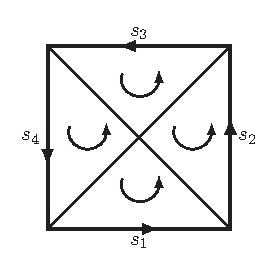
\includegraphics[width=50mm]{figures/3-2-1.pdf}\\图 3.2.1\end{center}
也可看正合列的一段 $H_2(K)\to H_2(K,K_0)\xrightarrow{\partial_*}H_1(K_0)\to H_1(K)$。因为 $|K|$ 可缩，两端群为零，故由引理 3.2.2(1)、(2)，中间映射为同构。

\entry{例}{3.2.10}图 3.2.2 中 $K$ 为环带，$K_0$ 为内外边界的并。例 1.10.5 已算过其相对同调，现在用正合列重算。
\begin{center}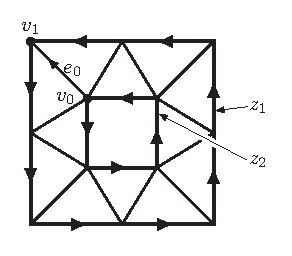
\includegraphics[width=52mm]{figures/3-2-2.pdf}\\图 3.2.2\end{center}
约化长正合列的一段为
\[
\begin{aligned}
0\to H_2(K,K_0)&\xrightarrow{\partial_*}H_1(K_0)\xrightarrow{i_*}H_1(K)\\
&\xrightarrow{\pi_*}H_1(K,K_0)\xrightarrow{\partial_*}\widetilde H_0(K_0)\to0.
\end{aligned}
\]
已知各群依次为 $0,\ ?,\ \Z\oplus\Z,\ \Z,\ ?,\ \Z,\ 0$。两端为零，因为 $|K|$ 与圆周同伦等价。$H_1(K)$ 可由绕外边界的 $z_1$ 或绕内边界的 $z_2$ 生成，两闭链同调。$K_0$ 为两个圆周的不交并，故 $H_1(K_0)$ 以 $\{z_1\},\{z_2\}$ 为基，而 $\widetilde H_0(K_0)\cong\Z$ 由 $\{v_1-v_0\}$ 生成。\translatornote{原文此处写作 $v_1-v_2$，但图中顶点为 $v_0,v_1$，后文边界也为 $v_1-v_0$。}

$i_*$ 将两基元素映到同一个生成元，所以它满射，其核由 $\{z_1\}-\{z_2\}$ 生成，为无限循环群。由满射性，$\pi_*=0$，故 $\partial_*:H_1(K,K_0)\to\widetilde H_0(K_0)$ 为同构。因此 $H_1(K,K_0)\cong\Z$，由边界为 $v_1-v_0$ 的链 $e_0$ 代表生成元。

另一方面，$\partial_*:H_2(K,K_0)\to\ker i_*$ 为同构，所以 $H_2(K,K_0)\cong\Z$。所有逆时针定向 $2$ 维单形之和 $\gamma$ 代表生成元，因为其边界在相差符号的意义下等于 $z_1-z_2$，代表核的生成元。

\sourcepage{157--158}
\entry{例}{3.2.11}同时考察两个例子：圆柱面及其上边界，或 Möbius 带及其唯一边界。两种情况下，$|K_0|$ 均为圆周，$|K|$ 也具有圆周同伦型。图 3.2.3 的中心圆周 $C$ 为形变收缩核。
\begin{center}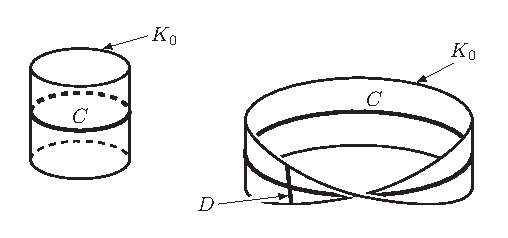
\includegraphics[width=91mm]{figures/3-2-3.pdf}\\图 3.2.3\end{center}
正合列相应片段的已知群为
\[
0\to H_2(K,K_0)\to\Z\xrightarrow{i_*}\Z\to H_1(K,K_0)\to0.
\]
关键是求 $i_*$。由于收缩 $r:|K|\to C$ 为同伦等价，只需求复合 $ri:|K_0|\to C$ 的作用。圆柱面情况下此映射的度为 $1$，而 Möbius 带情况下为乘以 $2$。所以圆柱面有 $H_2(K,K_0)=H_1(K,K_0)=0$；Möbius 带有 $H_2(K,K_0)=0$、$H_1(K,K_0)\cong\Z/2$。后一群的非零元素由中心圆周 $C$ 代表，也可由链 $D$ 代表，留作习题。

\subsection*{习题}
\begin{enumerate}
\item 验证引理 3.2.2 的 (1)--(5)。
\item \begin{enumerate}[label=(\alph*)]
\item 若 $A_i\xrightarrow{\alpha_i}B_i\xrightarrow{\beta_i}C_i$ 对 $i=1,2$ 均正合，证明乘积序列 $A_1\times A_2\xrightarrow{\alpha_1\times\alpha_2}B_1\times B_2\xrightarrow{\beta_1\times\beta_2}C_1\times C_2$ 正合。
\item 推广到任意直积。
\item 推广到任意直和。
\end{enumerate}
\item 若 $K_0$ 无环，证明 $H_i(K,K_0)\cong\widetilde H_i(K)$。
\item 若包含 $|K_0|\to|K|$ 为同伦等价，证明所有 $H_p(K,K_0)$ 为零。
\item 对例 3.2.11 的 Möbius 带偶，证明其非零相对一维同调类由图中的 $D$ 代表。
\item 设 $S$ 为 Klein 瓶，$A,C$ 为通常的简单闭曲线，见第 2.6 节习题 2。计算偶 $(S,A)$ 与 $(S,C)$ 的正合列。
\item 对正合列 $A\xrightarrow{\alpha}B\xrightarrow{\beta}C\xrightarrow{\gamma}D$，证明 $D\ne0$ 时 $\beta$ 不一定满射。
\item 对同一正合列，证明 $A\ne0$ 时 $\beta$ 不一定单射。
\end{enumerate}
